\documentclass[11pt]{jsarticle}

\usepackage{amsmath,amsthm,amssymb}
\usepackage[dvipdfmx]{graphicx}
\usepackage{bm}
%
\usepackage{multirow}
\usepackage{wrapfig}
%
\pagestyle{empty}
%% 高さの設定
\setlength{\textheight}{\paperheight}   % ひとまず紙面を本文領域に
\setlength{\topmargin}{-5.4truemm}      % 上の余白を20mm(=1inch-5.4mm)に
\addtolength{\topmargin}{-\headheight}  % 
\addtolength{\topmargin}{-\headsep}     % ヘッダの分だけ本文領域を移動させる
\addtolength{\textheight}{-40truemm}    % 下の余白も20mmに%% 幅の設定
\setlength{\textwidth}{\paperwidth}     % ひとまず紙面を本文領域に
\setlength{\oddsidemargin}{-5.4truemm}  % 左の余白を20mm(=1inch-5.4mm)に
\setlength{\evensidemargin}{-5.4truemm} % 
\addtolength{\textwidth}{-40truemm}     % 右の余白も20mmに

%
\abovecaptionskip=-1pt
%\belowcaptionskip=-1pt
%
\renewcommand{\baselinestretch}{0.94} % 全体の行間調整
\renewcommand{\figurename}{Fig.}
\renewcommand{\tablename}{Tab.}
%
\makeatletter 
\def\section{\@startsection {section}{1}{\z@}{1.5 ex plus 2ex minus -.2ex}{0.5 ex plus .2ex}{\large\bf}}
\def\subsection{\@startsection{subsection}{2}{\z@}{0.2\Cvs \@plus.5\Cdp \@minus.2\Cdp}{0.1\Cvs \@plus.3\Cdp}{\reset@font\normalsize\bfseries}}
\makeatother 
%

\begin{document}

%%%%%%
% はじめに
%%%%%%
\begin{center}
{\Large \textgt{12. MD シミュレーションによるネットワークポリマーのゴム弾性}}
\end{center}

\begin{flushright}
東亞合成 佐々木裕

Tel: 052-611-9923, e-mail: hiroshi\_sasaki$@$mail.toagosei.co.jp
\end{flushright}

\vspace{0.5\baselineskip}
\section{はじめに}
%\subsection{ネットワークポリマーのゴム弾性}
%
%一般にプラスチックと呼ばれる材料は熱可塑性の高分子材料であり、室温以上のガラス転移温度を有し固体材料として使用することができる。
%しかしながら、そのガラス転移点以上の温度においては巨視的な流動が生じて流れてしまうため、力学特性を利用した材料設計を行う場合に、ネットワーク構造の導入は非常に有効な手段の一つである。
%
%熱可塑性であるプラスチックとの対比から、ネットワークポリマーは熱硬化性樹脂として「硬い材料」と認識される場合も多いが、ネットワークが常に固いものであるとは限らない。
%その典型的な例として、柔らかさと強さを兼ね備えた旧知の材料であるゴムを挙げることができる。
%さらに、ある程度の高温までの広い温度範囲において硬い材料であり封止剤や接着剤に広く用いられているエポキシ樹脂のような材料であっても、ガラス転移温度以上ではゴム領域となりゴム弾性を示すのであるからその振る舞いを理解することは重要である。

\subsection{ゴム弾性理論}

ゴム弾性の最も古典的なモデルは、ネットワークを構成するストランドをガウス鎖と考え、その結節点のミクロな変形がマクロな変形度合いと相似であるアフィン変形するとした「アフィンネットワークモデル」である~\cite{Flory1953}。
このモデルから導出したもっとも単純な弾性応答モデルは、「ネオ・フッキアンモデル」であり、古典モデルとも呼ばれている。

古典モデルからの発展形として、主として二つの重要な考え方が提案されている。
一つは、結節点の揺らぎに注目したモデルであり、結節点がその平均の位置から自由に揺らぐとした「ファントムネットワークモデル~\cite{James1943}」、そして、ポリマー鎖の絡み合いにより結節点の揺らぎがある程度抑制される効果を考慮した「コンストレインド・ジャンクションモデル~\cite{Flory1982}」が知られている。
もう一つが、ストランドに Kuhn らが提唱した「鎖の伸びきり効果」を逆ランジュバン関数で表したモデル~\cite{Kuhn1942} を用いたものである。
ユニットセル中に八本のポリマー鎖を配置した「八本鎖モデル~\cite{Arruda1993}」、ランダムに配置された鎖が変形することを想定した「フルチェインモデル~\cite{Wu1993}」が提案されている。

\subsection{シミュレーションによる先行研究}

ポリマーの分子動力学(MD)シミュレーションでは、Kremer らが提唱したポリマー鎖のすり抜けを抑制し絡み合いを表した 「KG 鎖」と呼ばれるビーズ・スプリングモデル~\cite{Kremer1990} が、実在鎖との整合性がよいモデルとして広く用いられている。
また、ビーズ間のポテンシャルを省略してポリマー鎖のすり抜けを許容したポリマー鎖は「ファントム鎖」と呼ばれている。

Everaers らは、規則構造を有するネットワークを用いて、「KG 鎖」と「ファントム鎖」との比較を行い、各種のゴム弾性理論との高い整合性を報告している~\cite{Everaers1999}。
この検討においては規則的なネットワーク構造に起因したノーマルモードがみられ、すり抜けを許容した「ファントム鎖」においてもアフィン変形する「ネオ・フッキアンモデル」としての挙動を示すことが確認されている。

\subsection{本検討内容}

我々は、規則構造ネットワークのユニットセル間における規則性をランダムへと変えてノーマルモードを抑制することで、結節点の揺らぎに由来する「ファントムネットワークモデル」の構築を検討した。

本報告では、平衡構造での鎖の挙動、及び、大変形時の挙動に注目した検討結果について報告する。

\section{シミュレーション}

ランダムな結合性を有するネットワークを作成し、その平衡状態および一軸伸長時の振る舞いについて、OCTA 上の COGNAC シミュレーターを用いた分子動力学シミュレーションにより評価した。

\subsection{ネットワークモデルの作成}
N 個のビーズからなるストランドを用いて、体心立方構造の各格子点をストランドでつないだ「八本鎖モデル」のユニットセルを作成し、その連なりとしてネットワークの初期構造を表した。

以下のアルゴリズムで各ノードの隣接関係にランダム性を導入した。

\vspace{-3mm}
\begin{enumerate}
\item
実空間で初期構造(ストランドの末端間距離をメルトと同一と設定)の作成。
\item
初期構造に対応したトポロジーモデルを用いて、ノードごとのエッジ数(分岐数)に変換。
\item
そのトポロジーモデルに対応するように、実空間の初期構造からストランドを除去。
\item
複数のネットワークが相互貫入した IPN 構造の多重度(Multi)を設定。
\end{enumerate}
\vspace{-3mm}
%こうすれば、実空間で遠く離れたノードをつなげることを抑制できた。

%\renewcommand{\arraystretch}{1.5}
%\begin{wraptable}{r}{60mm}
%%\vspace{-0.5\baselineskip}
%	\caption{Network Model}
%	\label{tbl:Network Model}
%	\centering
%	\footnotesize
%	\begin{tabular}{ c c c c} \hline
%	Seg./Str. 	& Multi	& Cells					& $\nu$		\\ \hline \hline
%	44		& 9 	& $2\times2\times2$ 	& 0.020		\\ \hline
%	\end{tabular}
%\vspace{-2mm}
%\end{wraptable}



\begin{wrapfigure}{r}{60mm}
\vspace{-1\baselineskip}
	\begin{center}
	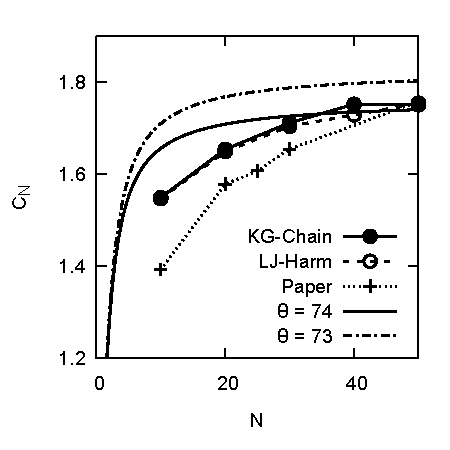
\includegraphics[width=60mm]{./fig/C_ratio.pdf}
	\caption{Characteristic Ratio for varied length of KG Chains and others}
	\label{fig:Characteristic Ratio}
	\end{center}
%\vspace{-10mm}
\end{wrapfigure}

\subsection{ポテンシャルの設定}

KG 鎖は、非結合ポテンシャルとして各ビーズ間に LJ ポテンシャル $U_{LJ}(r)$、ボンドポテンシャルに FENE-LJ ポテンシャル $U_{FENE}(r)$ を用い、ファントム鎖は非結合ポテンシャルを省略した。

\section{結果と考察}

\subsection{特性比の振る舞い}

セグメント数 $N$ の異なる ``KG Chain'' のメルト状態での特性比($C_N$)を Fig.\ref{fig:Characteristic Ratio} に示した。
線形バネモデルでは、$R_0=1.0, K=100$ とした場合にほぼ同じ挙動となった。
これらのシミュレーションにおいては、セグメント間の斥力のため、ボンド長は 0.97 程度に圧縮されていた。

また、自由回転鎖モデルからの理論線では $N$ の大きな領域で、$\theta \simeq 74$ に漸近した。





\begin{wrapfigure}{r}{60mm}
\vspace{-3\baselineskip}
	\begin{center}
	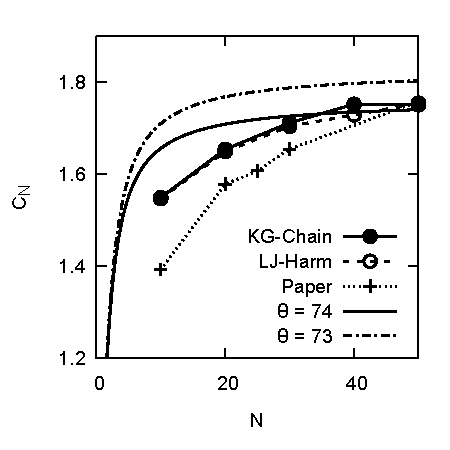
\includegraphics[width=60mm]{./fig/C_ratio.pdf}
	\caption{Characteristic Ratio for varied length of KG Chains and others}
	\label{fig:Characteristic Ratio}
	\end{center}
\vspace{-10mm}
\end{wrapfigure}

\subsection{鎖の交差}

``KG Chain'' での鎖の交差ポテンシャル $U_{cross} \simeq 70 k_B T$ と見積もれ、通常の条件では鎖の交差が生じないとされる。

非結合ポテンシャル $U_{LJ}(r)$ と線形バネポテンシャル $U_{Harm}$ との組み合わせでは、自然長 $R_0$ とバネ定数 $K$ の適切な設定によりこの値を小さくできる。

\subsection{一軸伸長}
``KG Chain'' からなるダイヤモンドネットワークの一軸伸長($10^{-5}\lambda/\tau$)時の SS カーブを、Fig. \ref{fig: stretch} に示した。


$\lambda<2$ 程度の小さなひずみではネオフッキアンモデルに合致した。
しかし、大変形領域においては、特性比より算出したクーンセグメント数($N_K\simeq 16.6$)に換算した場合には、対応した伸びきり鎖の応力モデル~\cite{Arruda1993}とは合致せず、$N=21$ 程度でフィットできたため、伸長時には平衡状態のアングルから伸びているものと推測できた。



%\begin{wrapfigure}{r}{60mm}
%\vspace{-4\baselineskip}
%	\begin{center}
%	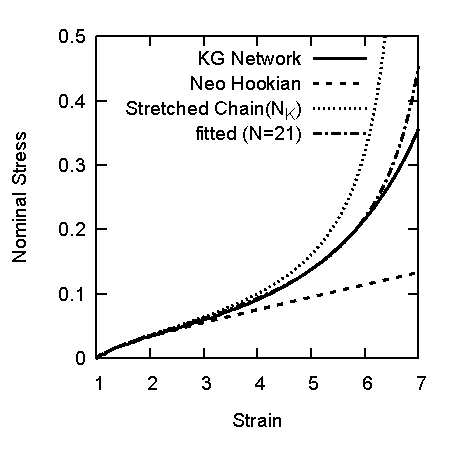
\includegraphics[width=60mm]{./fig/SS.pdf}
%	\caption{Uniaxial Elongation SS Curve and Energies Result with Stretched Chain Model~\cite{Arruda1993}}
%	\label{fig: stretch}
%	\end{center}
%%\vspace{-40mm}
%\end{wrapfigure}



\bibliographystyle{achemso}
%{elsart-num}
%{junsrt-2}
\bibliography{./library.bib}

\end{document}